\documentclass[prodmode,hillsideplop]{acmlarge}
\usepackage[utf8]{inputenc}
\usepackage{flafter}
\usepackage{hyperref}
\usepackage[hyphenbreaks]{breakurl}
\usepackage{pdflscape}
\usepackage{framed}
\usepackage{caption}

% Metadata Information
\acmVolume{22}
\acmYear{2015}
\acmMonth{10}

% Package to generate and customize Algorithm as per ACM style
\usepackage[ruled]{algorithm2e}
\SetAlFnt{\algofont}
\SetAlCapFnt{\algofont}
\SetAlCapNameFnt{\algofont}
\SetAlCapHSkip{0pt}
\IncMargin{-\parindent}
\renewcommand{\algorithmcfname}{ALGORITHM}


% Page heads
\markboth{P. Silva, R. Monge and E B. Fernandez}{A Reference Architecture for web browsers: Part III, A pattern for a Web Browser Kernel}

% Title portion
\title{A Reference Architecture for web browsers: Part III, A pattern for a Web Browser Kernel.}
\author{
%\alignauthor
Paulina Silva and Raúl Monge
  \affil{Universidad Técnica Federico Santa María}
  %\affil{Valparaíso, Chile}\\
  %\email{pasilva@alumnos.inf.utfsm.cl}
% 2nd. author
%\alignauthor
  %\affil{Valparaíso, Chile}\\
  %\email{rmonge@inf.utfsm.cl}
% 3rd. author
%\alignauthor 
Eduardo B. Fernandez
  \affil{Florida Atlantic University}
  %\affil{Boca Raton, Fl, USA}\\
  %\email{fernande@fau.edu}
}

\appendixauthor{IF DIFFERENCE AUTHORS INCLUDE HERE, University of New Hampshire}

\begin{abstract}
Web browsers are a fundamental component of the Internet and have a critical value for security. Since 2000 a number of new browser designs have appeared, since the monolithic architecture used before had not considered some important design decisions, like security, stability and others. New Web Browser architecture designs are likely to be based on operating systems properties where several cooperative processes use the same process structure used by operating systems to implement system services. A \textbf{Web Browser Kernel} is the main component representation in charge of controlling what the browser does, like an operating system. It communicates with other processes, its child processes, and sends instruction to them; of course, according to the \textbf{Browser User}’s will. A \textbf{Web Browser Kernel} is a piece of software that could be found whenever we are using a \textbf{modular architecture} in a Web Browser. The pattern we are developing on this paper has abstracted a part of the internals of the Web Browser, and we show what happen when the user asks for content to be display into the screen of a Web Browser host.

\end{abstract}

\category{}{}{}[]
\category{}{}{}[]
\category{}{}{}[]

\keywords{Browser, Web Client, Browser Renderer, Reference Architecture, Pattern}
\acmformat{Paulina Silva, Raul Monge, and Eduardo B. Fernandez. A Reference Architecture for web browsers: Part III, A pattern for a Web Browser Kernel}

\copyr{PLoP'X, asdf. Copyright 201X is held by the author(s). {HILLSIDE}}

\begin{document}

% Metadata Information
\acmVolume{X}
\acmYear{Y}
\acmMonth{2017}

\begin{bottomstuff}
Permission to make digital or hard copies of all or part of this work for personal or classroom use is granted without fee provided that copies are not made or distributed for profit or commercial advantage and that copies bear this notice and the full citation on the first page. To copy otherwise, to republish, to post on servers or to redistribute to lists, requires prior specific permission. A preliminary version of this paper was presented in a writers' workshop at the 2Yth Conference on Pattern Languages of Programs (PLoP).
\end{bottomstuff}

\maketitle

\section{Introduction}
We are currently developing a serie of architectural patterns to build a Reference Architecture (RA) and Security Reference Architecture (SRA) for a Web Browser \cite{silva2015,silva2015b,silva2016a}.
An RA is an abstract architecture that describes functionality without getting into implementation details. Its aim is to provide a guide to build architectures for concrete versions of some system or to extend such system \cite{Avgeriou2003,Galster2011a,Angelov2012}.
A SRA on the other hand, provides information about possible threats and defense mechanisms of the system. Based on work in \cite{Fernandez2006}, they proposed an approach for building SRAs using patterns, where they defined a precise and semiformal security cloud computing architecture for the complete cloud environment \cite{Fernandez2016}. They showed that SRAs are useful to apply security to cloud systems and for a variety of other purposes. Our intent in describing the Web Browser as a RA and SRA is to understand the symbiosis between the client and the Web Server to which the user asks for resources, and the related security implications. Because we know that a client would not exist without its counterpart, the server, we think that security must be seen and understood from both sides and not only on the server side like most developers do \cite{alcorn2014browser}.
We have used patterns in our work because they encapsulate solutions to recurrent problems and define a way to concisely express requirements and solutions, as well as providing a communication vocabulary for designers \cite{gamma1994design,buschman1996system}. The problem ...agregar algo... is not a single problem like in traditional design patterns but it is a composite objective. In fact, our three patterns are composite patterns, which pursue more than one objective, or perhaps one objective by combining several partial solutions, which combinated create are RA. The description of architectures using patterns makes them easier to understand, provides guidelines for design and analysis, and can define a way of making their structure more secure. We have looked at several browsers, like Google Chrome, Firefox and Internet Explorer (Edge). We do not say that this is the optimal or the only solution for this problem. But this solution is representative of several browsers and it is a generic solution that can be used again.
 

\begin{figure*}[h!t]
  %\vspace*{-0.4cm}
  \centering
  %\hspace{0.5cm}
  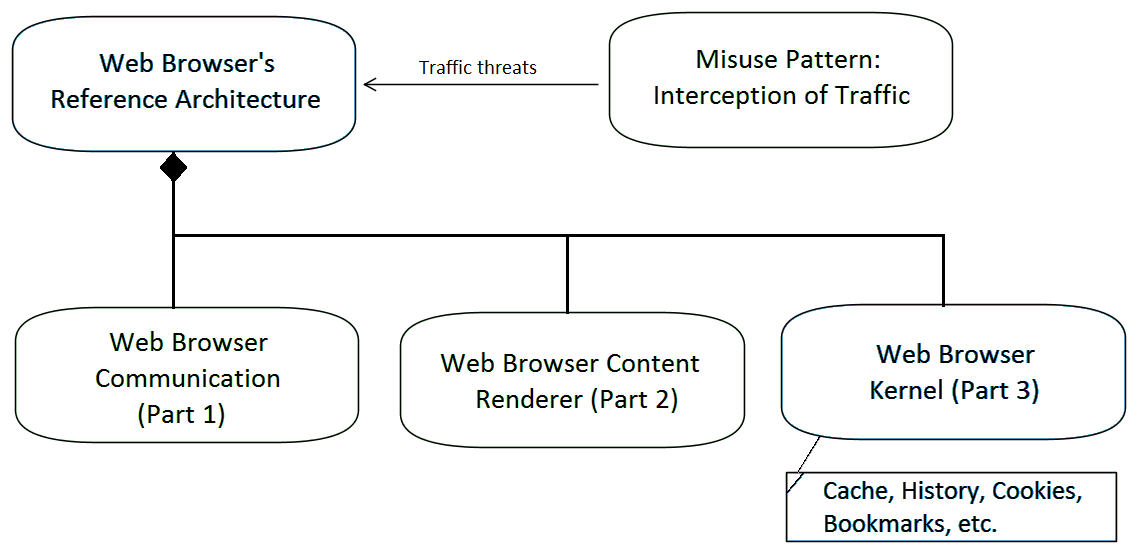
\includegraphics[scale=0.3]{imgs/relations-finish.png}
  \caption{Pattern Diagram of our current work on the Reference Architecture for the Web Browser.}
  \label{fig:pattDiag}
\end{figure*}
\vspace*{-0.3cm}

\begin{figure*}[h!t]
    \vspace*{-0.5cm}
    \centering
    \hspace{0.5cm}
    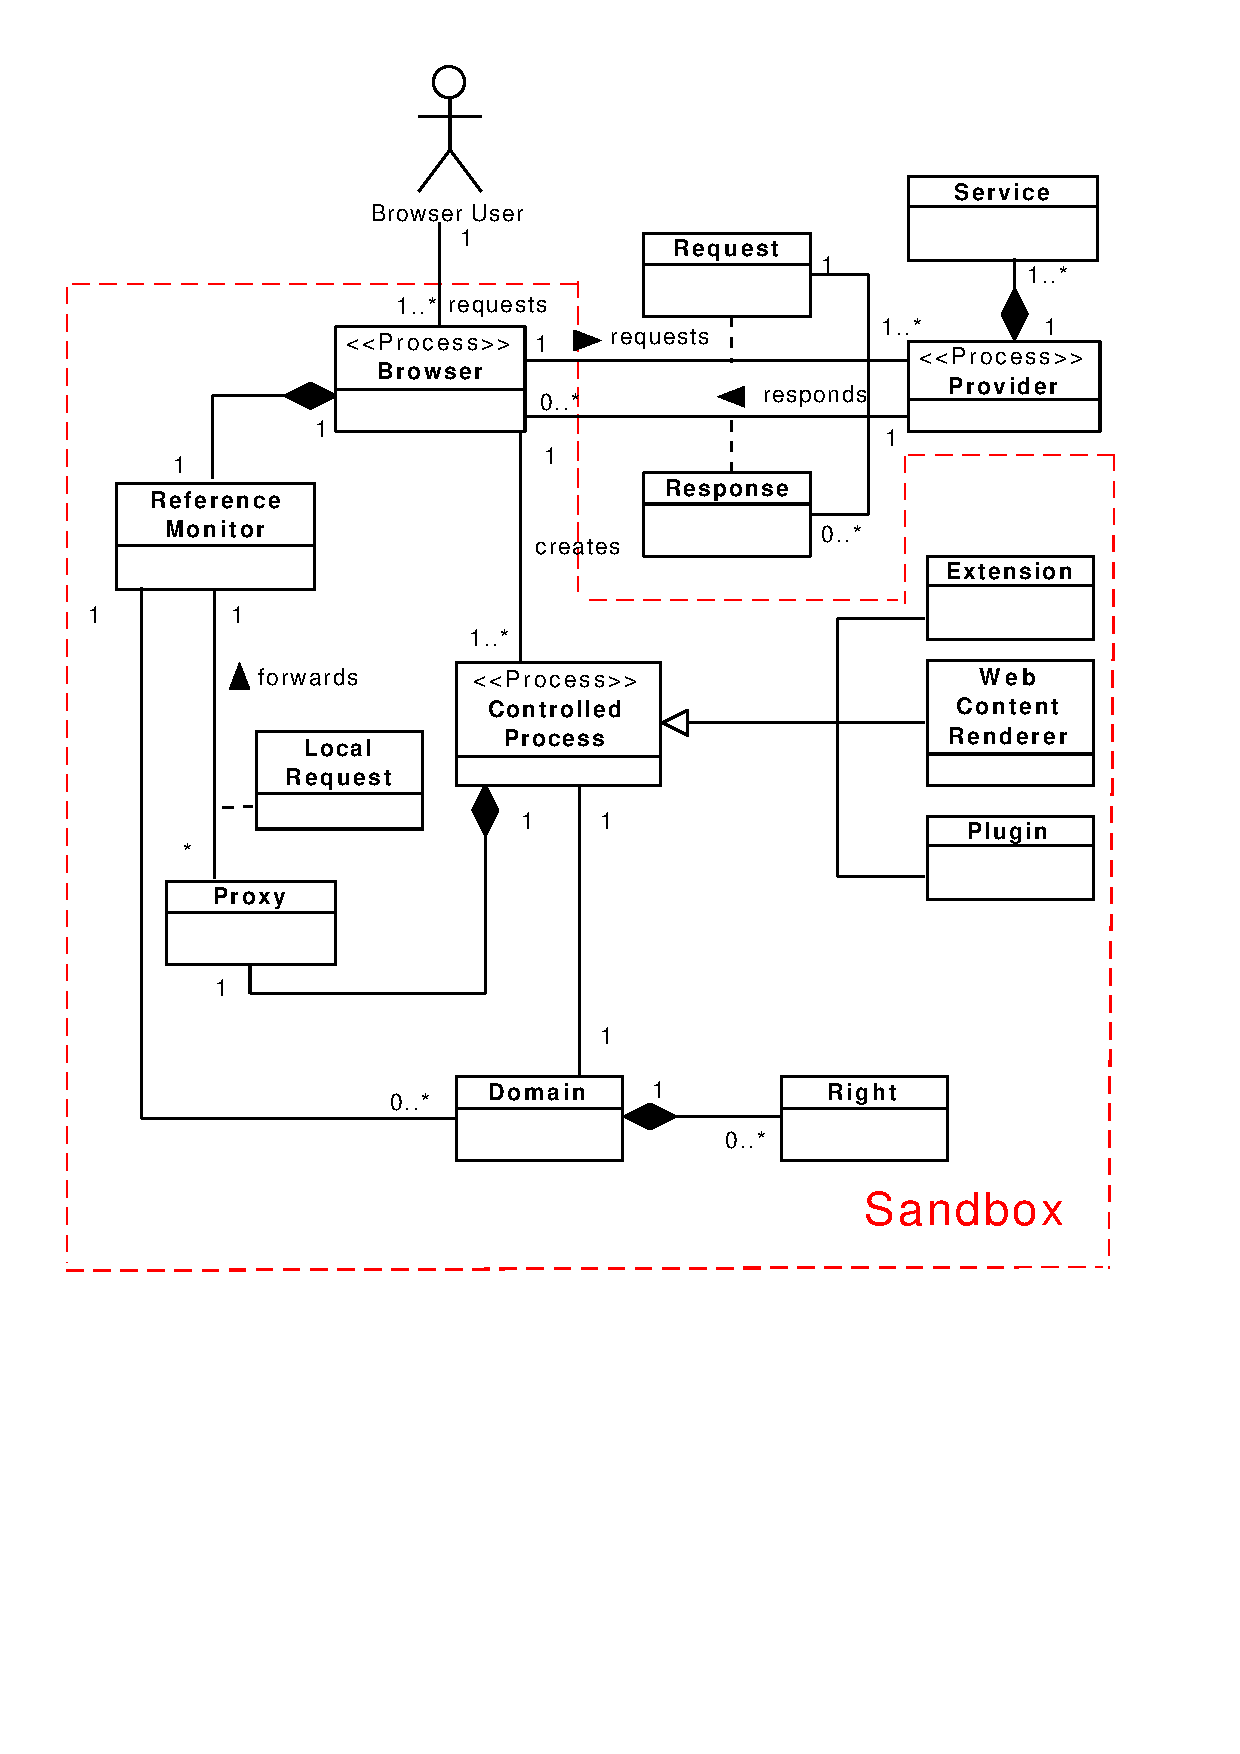
\includegraphics[scale=0.52]{imgs/WBC.pdf}
    \vspace*{-3.5cm}
    \caption{Overview of the high component for a Web Browser}
    \label{fig:BInfra}
\end{figure*}
 In previous work \cite{silva2015,silva2016a}, we use a pattern diagram \cite{Fernandez2008} (Figure \ref{fig:pattDiag}) to show the relationships between our patterns and we can see how they relate to each other (rounded rectangles represent patterns and the arcs indicate dependencies between patterns). Figure \ref{fig:BInfra} \cite{silva2015} shows an overview of the high level components of a Web Browser and how they are related with the current pattern, \textbf{Web Browser Kernel}.
\section{Web Browser Kernel}
\subsection{Intent}
In its modular architecture, the Web Browser Kernel is the main control point of a browser. It establishes and orchestrates the control and communications channels among the other components of the browser to satisfy the needs of a Browser User (Figure \ref{fig:BK}).


\subsection{Example}
%A Browser User wishes to request a varieties of web pages in different sites. Some of these resources could be web pages already seen and some of them new pages; the client in this case, tries to comply with the Browser User’s requests as fast as it can. While some of these requested resources can be easily shown to others, the browser may need to be authenticated to the Web Server where the resource is hosted. The Web Browser should have basic communication to all possible web servers on the Internet, and provide security for the Browser User’s own data as well as the server's data.

When a user launches a browser, a user interface must be displayed and the components subsystems  of a browser need to be instantiated and wired together so they are ready to respond to user input and provide the functionality of web browsing. 

\subsection{Context}
A Web Browser is a client which searches for resources on any Web Server connected to the Internet. The Web Browser main control point organizes a set of functional subsystems that collectively implements browsing features. Each Web Browser component communicates via various communication channels that can be configurated as needed. To display requested resources, Web Browser components must have enough allocated systems resources; faults in components can also occur and should be deactivated.

\subsection{Problem}
A Web Browser is constantly being asked by the Browser User for resources on the Internet. If the Web Browser has a monolithic architecture, it may not be able to satisfy all the requests and sometimes they could fail, making the Web Browser crash or become unusable. How can a Web Browser be prepared for these events?

The solution to this problem must resolve the following forces:

\begin{itemize}
	\item \textbf{Compatibility:} a Web browser should comply with web standards for a correct implementation and display of the content.
    \item \textbf{Compartmentability/Isolation:} A Web Browser should be able to show all the content, even when a page could be broken and have errors. The Web Browser should keep on browsing even after problems arise on a web page, were it should not be reflected on other rendered web pages.
    \item \textbf{Speed:} A web page should be displayed to the Browser User as fast as possible and respond to user's interaction as quickly as possible to ensure a better browsing experience.    
    \item \textbf{Security:} The user's and server’s information should be kept secure under any circumstances (privacy of data also is included).
    
\end{itemize}

\subsection{Solution}
Since a monolithic architecture concentrates all the work a Web Browser does on a single process, a better solution is to have a modular architecture \cite{Vrbanec2013,Wu2014,barth2008security,reis2009browser}, where a process is only in charge of requesting resources and delegates the rendering work to its children (or renderer) processes. The Web Browser Kernel acts as the parent process of the browser and will work with the Web Browser Content Renderer \cite{silva2015} instances to display accordingly the content being asked. Based on the same principles a operating system has like, separation of concerns, compartmentalization, least privileges, the Web Browser with a modular architecture will be able to contain the propagation of rendering errors and the consequences of unexpected or malicious behaviour.

\begin{figure*}[h!t]
  \vspace*{-0.5cm}
  \centering
  %\hspace{0.5cm}
  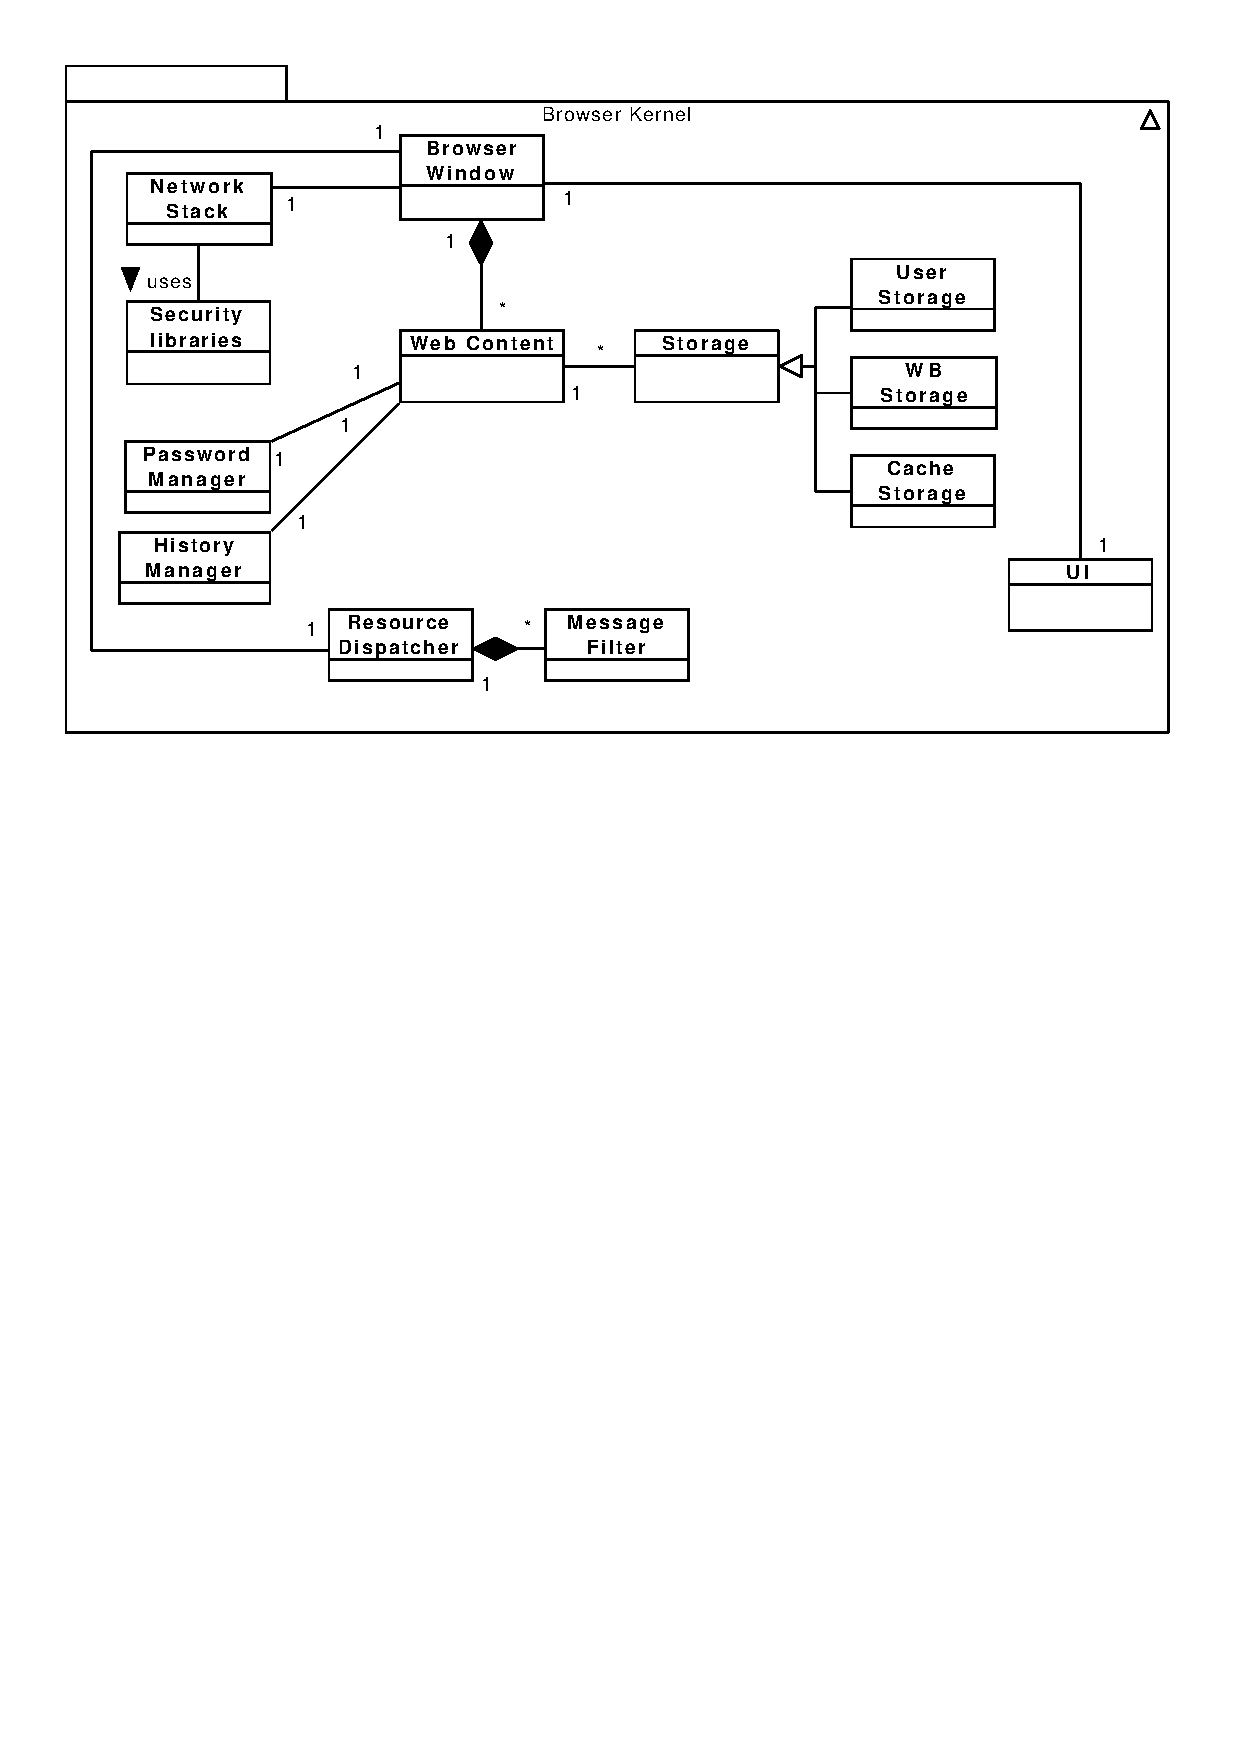
\includegraphics[scale=0.7]{imgs/WBK.pdf}
  \vspace{-11.5cm}
  \caption{Pattern for our Web Browser Kernel}
  \label{fig:BK}
\end{figure*}

\subsubsection{Structure}
Figure 2 shows a class diagram for the \textbf{Web Browser Kernel} pattern. The browser host machine receives user’s interactions from input devices like mouse or keyboard. When a url is prompted from the \textbf{Browser User}, the windows manager of the host machine delegates this action to the \textbf{UI} of the Web Browser. The \textbf{Browser Window} searches in the \textbf{Browser’s Storage} for an old version of the page, on the cache. If no old copy of the page from the url being ask is found, an implementation of the \textbf{Network Stack} is used to make system calls for the url being asked. \textbf{User Storage} is used to complete with user's information in the outgoing request, like adding cookies, etc. \textbf{Web Browser Storage} is in charge of storing binaries or files downloaded by the Web Browser. \textbf{Security libraries} are implemented on the browser and are used to encapsulate requests to make sure they become secured to the server hosting the resource the \textbf{Browser User} wants. The \textbf{Password Manager} is in charge of securing old passwords from the \textbf{Browser User} and use them in case there are needed. \textbf{History Manager} saves all past requests from the \textbf{Browser User}, and lets its users modify it at will. When the request is finally encapsulated to make the request to a server, sockets from the operating system will be used to send the request to the Web Server of interest. Once a response to the sent request comes back to the host machine, the \textbf{Browser Kernel} will receive it and the \textbf{Browser Window} will use the \textbf{Resource Dispatcher} to send it it to a new or old \textbf{Web Browser Content Renderer} \cite{silva2015,silva2016a}, thanks to the \textbf{Message Filter}. 

\subsubsection{Dynamics}
Some use cases are the following:
%[usar paper que encontré sobre los caso de uso del WB] 
  \begin{itemize}
      \item Content Retrieval
      \item Save to storage: cache, Web Browser data or user data
      \item Manage bookmarks
      \item Monitor Web Browser
      \item Receive user input
      \item Send content to render
  \end{itemize}
We show in detail Content Retrieval below, since is the most important use case for the Web Browser.

\subsubsection{Summary}
The Browser User asks for the content indicated by the URL typed on the keyboard and pushes enter to access the resource, or interacts with an already loaded resource on the Web Browser.

\subsubsection{Actor}
Browser User

\subsubsection{Preconditions}
The host machine must have one or more \textbf{Web Browser Kernels} for the \textbf{Browser User}, and should be connected to a network or the Internet. The provider the user wants to contact must also be available.

\subsubsection{Description}
The \textbf{Web Browser Kernel} is the representation of the main process, or parent process, for a Web Browser with modular architecture. When a \textbf{Browser User} surfs through the Internet, the \textbf{Web Browser Kernel} receives through the Web Browser’s host machine the necessary input, like user interface interaction through the keyboard or the mouse.

\begin{figure*}[h!t]
  %\vspace*{-0.4cm}
  \centering
  \hspace{-2cm}
  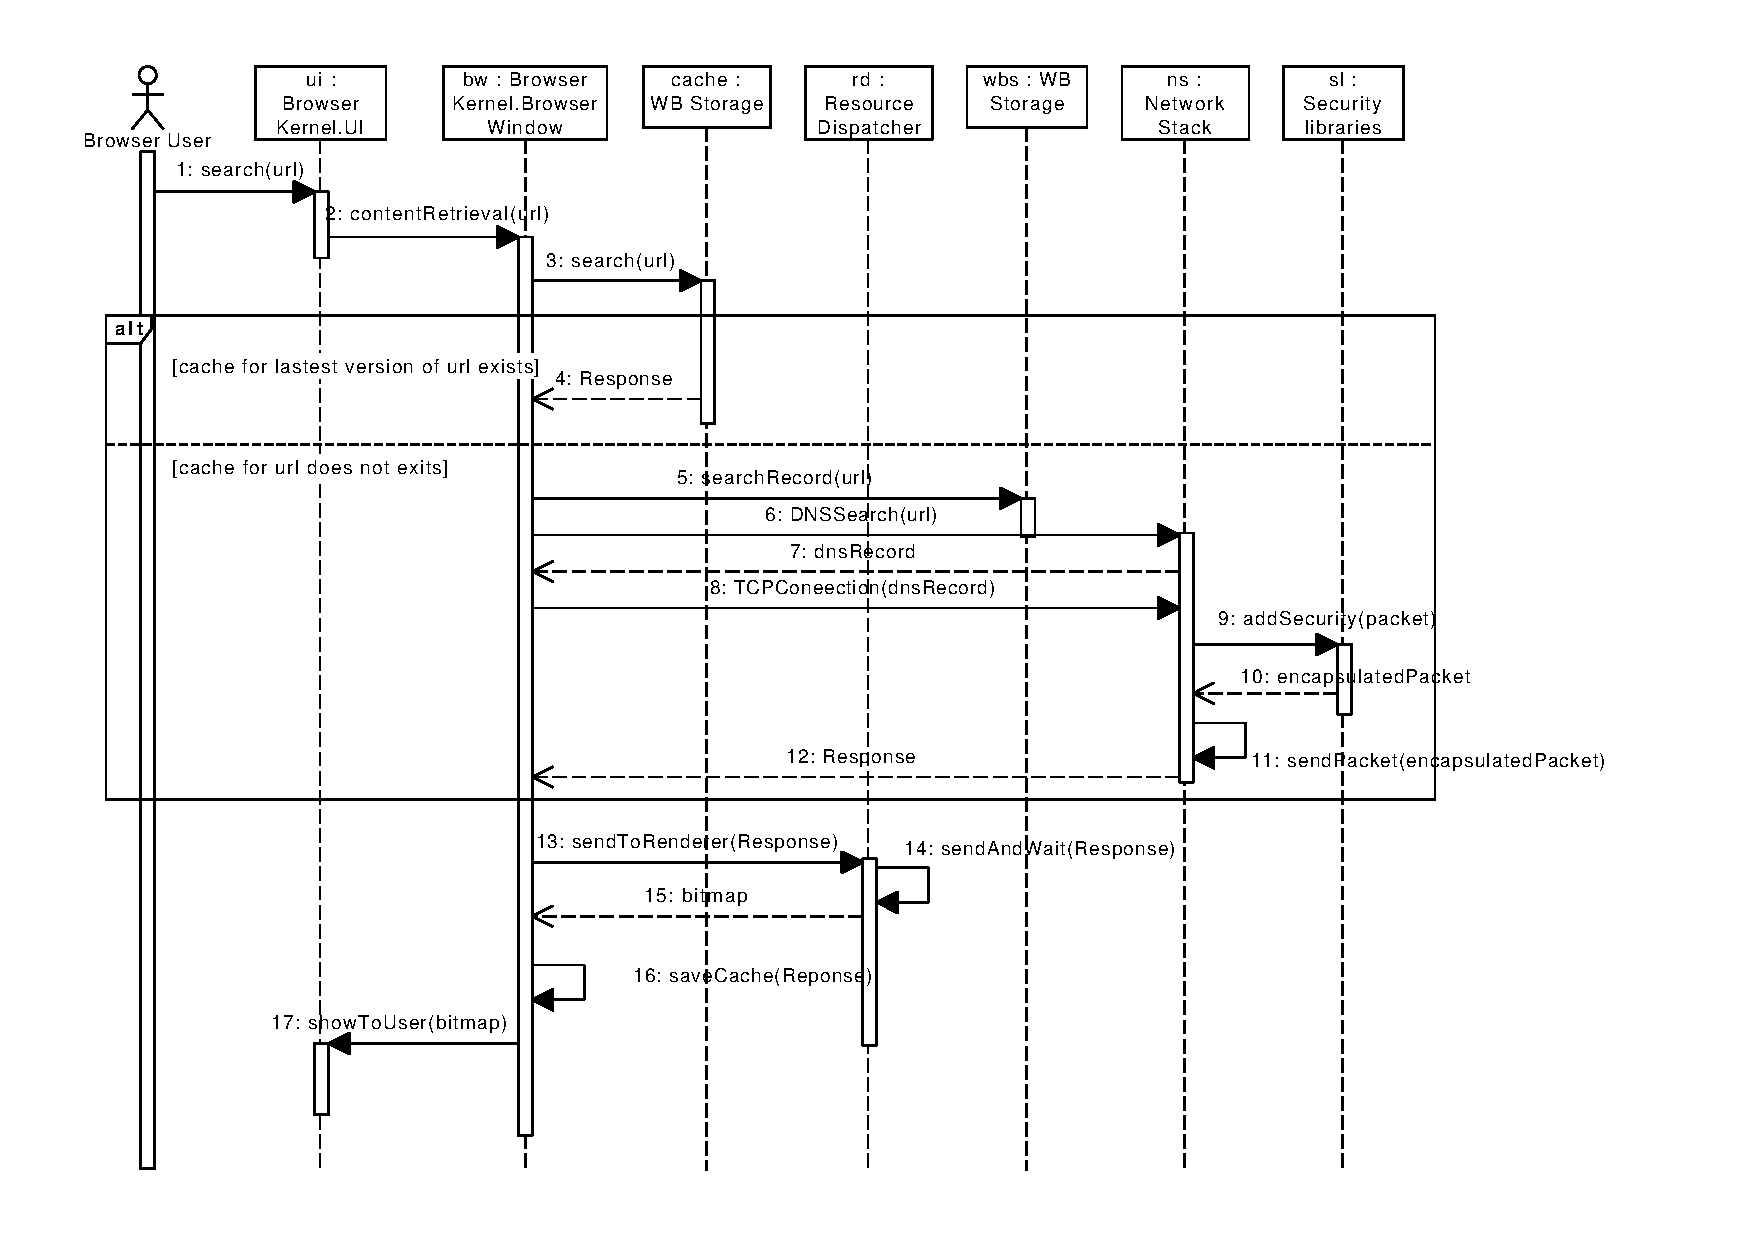
\includegraphics[scale=0.63]{imgs/contentRetrieval.pdf}
  \caption{Dynamics for: Content Retrieval}
  \label{fig:BK}
\end{figure*}

\begin{enumerate}
	\item A \textbf{Browser User} that wishes to retrieve content, interacts with the Web Browser and this interaction is received by the interface provided by the \textbf{Web Browser Kernel's UI}, which receives in this case the url of the page the \textbf{Browser User} wishes to see.
    \item The \textbf{Browser Window} is in charge of coordinating the \textbf{Web Browser Kernel} process and receives input from users with the help of its UI.
    	\begin{enumerate}
    		\item  Before searching the content on the Internet, the Web Browser will search on its cache if a recent data on the requested url has been saved. If the content is available and up to date, the Web Browser will render it. Go to step 3.
            \item If the Web Browser did not find anything for the asked url.
              \begin{enumerate}
              	\item  The \textbf{Browser Window} will ask the \textbf{Browser Storage} for the \textbf{Browser User}’s credentials if needed and will ask the \textbf{Network Stack} for a DNS search for the url.
                \item If a record is found for the url asked, a TCP connection is made to the \textbf{Network Stack}; including the necessary credentials for the request . Depending on the request, \textbf{Security Libraries} could be used on the request, to encapsulate data and send it securely.
                \item When the \textbf{Network Stack} sends the request, if a response is received, this is given to the \textbf{Browser Window}.
              \end{enumerate}
    	\end{enumerate}
	\item Wherever the response came from, let be from the cache or a up-to date server’s response, the \textbf{Browser Window} will send the response to the \textbf{Resource Dispatcher}. The latter is in charge of sending the soon-to-be rendered page, but before doing it the dispatcher uses its \textbf{Message Filter} to send it to the right \textbf{Controlled Process} \cite{silva2015}.
    \item After the Controlled Process, instantiated as a Web Browser Content Renderer, sends the bitmap for the resource obtained by the request from the Browser User, the Browser Window will save the rendered web page.
    \item Finally, the Browser Window sends to the User Interface the bitmap to be shown by the display of the Browser User’s machine.

\end{enumerate}

\subsubsection{Alternative Flows}
\begin{itemize}
	\item The resource obtained is not a web page, it could be a binary or a file. In this case, instead of rendering the response, the Web Browser only downloads it.
   \item The resource pointed by the URL does not exists.
   \item The request is cancelled.

\end{itemize}

\subsubsection{Postconditions}
The Browser receives the resource indicated by the URL and it is displayed by the peripheral device output for the Browser User.

\subsection{Implementation}
\begin{itemize}
	\item The Same Origin Policy (SOP) \cite{Zalewsk082} is defined by the origin, and is used to separate different resources by its domain, scheme and port. It is the minimum security mechanism a browser has while requesting cross-origin resources, and divides the different kinds of contents so they cannot interfere with each other. To enforce the Same Origin Policy, Google Chrome, Firefox and Internet Explorer use different schemes \cite{Barth2010,Grier2008} [add more references];for example, Google Chrome leaves pages/resources isolated with the help of the Renderer. The Resource Dispatcher with the help of its Message Filter does the job of receiving correctly different requests from the Controlled Processes instantiations.
    \item The SSL/TLS protocol complements this pattern while providing security (using the Security Library class) for communication channels between the browser and the provider. The Security Library class in our pattern makes this happen.
\end{itemize} 

\subsection{Consequences}
The Browser Kernel pattern provides the following benefits:
\begin{itemize}
	\item \textbf{Compatibility:} By using Web Standards a web developer assures that the content is shown as she expected.
        \item \textbf{Compartmentability/Isolation:} Since a modular architecture is used, web pages are rendered through children \textbf{Controlled Processes} which are \textbf{Web Browser Content Renderer} instantiations \cite{silva2016a}. Even thought child process can interact through the \textbf{Web Browser Kernel}, all the rendering is isolated in the child and will not interfere with other children and the main processes.
        %A Web Browser should be able to show all the content, even when a page could be broken and have issues. Problems on a web page should not be reflected on other rendered web pages.
    \item \textbf{Speed:} Since the work is distributed through the \textbf{Web Browser Kernel} and the \textbf{Web Browser Content Renderer} instantiations, speed is increased if compared with a monolithic architecture.
    %A web page should be displayed to the Browser User as fast as possible.    
    \item \textbf{Security:} Browser User's Information remain only accessible to the \textbf{Web Browser Kernel} only. If needed to surf on the Internet, it will be only used by the main process. In a way that the main process is isolated from its children processes or \textbf{Web Browser Content Renderer} instantiations, through the calls that are allowed to enter to the main process; the \textbf{Message Filter} is in charge of this.
    %The user's and server’s information should be kept secure under any circumstances (privacy of data also is included).
\end{itemize}
This pattern has the following liabilities:
\begin{itemize}
	\item Resources from Providers which do not comply the specifications of the W3C, will be displayed incorrectly by the Web Browser.
    \item Session Cookies that will be stored on the Browser Storage will be the Achilles heel for the Web Browser. Even if they provide us with a stateful communication, they can affect tremendously the Browser User and the Provider on the Internet by becoming attack vectors for XSS or CSRF attacks, whenever a Web Browser has exploitable vulnerabilities or bad implemented functions.
\end{itemize}


\subsection{Example Resolved}
With the pattern of the modular architecture for the Web Browser here presented, the browser will posses a more stable, fast and secure architecture, which will let show all the Browser User's requested web pages. This is possible because the Web Browser will not break if one page could not be displayed as instructed or will not be paused completely if a Web Server is not answering. As we have defined before, the Browser Kernel is essentially the controller of the browser, and delegates the hard work - rendering - to its children processes.


\subsection{Known Uses}
\begin{itemize}
	\item Google Chrome is based on a modular architecture, where a Browser Kernel acts as the main process of its Web Browser Chrome and Chromium (Open Source) \cite{barth2008security}. 
    \item Internet Explorer and Edge are proprietary browsers, which do not give much information about their structure or implementation. \cite{Crowley2010,IE8LCIE2} address the Loosely-Coupled architecture of Internet Explorer which is also a modular architecture.
	\item Firefox \cite{firefoxMulti}

\end{itemize}

\subsection{Related Patterns}
\begin{itemize}
	\item The Web Browser Communication pattern presents the components of the Web Browser and how they communicate with each other when a resource is requested \cite{silva2015}.
    \item The Web Browser Content Renderer pattern describes at a high-level the components of a web renderer of a Web Browser. It is in charge of composing and obtaining bitmaps of the requested web resources \cite{silva2016a}.
    \item The Reified Reference Monitor \cite{fernandez2013security}, describes how to enforce authorization rights when a subject requests access to a protected object or service and returns a decision (response).
\end{itemize}


\subsection{Conclusion and Future Work}
When building web applications that connects users to services by using web browsers, some developers do not understand the symbiosis between the web client or browser and the web servers to which resources are being requested. %For users and organizations to be secure of their transactions over the Internet, developers should carefully understand the implications when the Web Browser is connecting and displaying a web page.
A Web Browser is a complex software and web application developers need to understand the basics of how a Web Browser works, what components make this web client and the interactions between them inside the Web Browser, and the mechanism involved in: (1) the communication with the Web Browser and Web Server and (2) how a web page is rendered. Our aim with this and our previous work is to make understandable the internals of the browser and the already said mechanisms by using architectural patterns to construct a Reference Architecture (RA) for web browsers. Our RA has been formulated with the \textbf{Web Browser Communication} pattern, the \textbf{Web Browser Content Renderer} and now the \textbf{Web Browser Kernel}. These three patterns abstract the infrastructure of a Web Browser to help others understand holistically the components, interactions and relationships of this system called Web Browser. We plan to build more patterns for the Web Browser, as a way to educate developers and stakeholders of web applications. 
%From these patterns possible security threats could be found by analyzing its activities (and use cases) \cite{braz2008eliciting}, and for each of this possible security threats in the system countermeasures to prevent or foresee such threats, through security patterns on the reference architecture, will be needed; Hence, the final work is to obtain the construction of a Security Reference Architecture for the browser. An example of the type of work to be carried out can be seen in \cite{Fernandez2016}. 
For basic Web Browser-to-server communication, the browser needs the basic tools to: obtain, translate and paint the contents a browser user wants to see, otherwise is not what we would call a "Web Browser". The Web Browser Kernel pattern summarizes the basic components a Web Browser has and use when trying to comply requests, as well as is introduced as the main control point for all the Web Browser user's actions. 


%The problem is not a single problem like in traditional design patterns but it is a composite objective. In fact, our three patterns are composite patterns, which pursue more than one objective, or perhaps one objective by combining several partial solutions.

%We are emphasizing core problems that appear in all browsers. This does not preclude the possibility of variants that optimize different  objectives.

%We have looked at several browsers, not just Chrome (please see 'Known Uses' in the paper). We do not say that this is the optimal or the only solution for this problem. But this solution is representative of several browsers and it is a generic solution that can be used again. 

%Our RA is itself a pattern and can be used as a guideline for building new browsers or evaluate existing browsers. In fact, there are few explanations of the existing browsers and our work should help in making this architecture explicit and open to improvements. 

%\subsection{Acknowledgements}

\bibliographystyle{ACM-Reference-Format-Journals}
\bibliography{refTodas_all}





\end{document}

